\documentclass{sigchi-ext}
% Please be sure that you have the dependencies (i.e., additional
% LaTeX packages) to compile this example.
\usepackage[T1]{fontenc}
\usepackage{textcomp}
\usepackage[scaled=.92]{helvet} % for proper fonts
\usepackage{graphicx} % for EPS use the graphics package instead
\usepackage{balance}  % for useful for balancing the last columns
\usepackage{booktabs} % for pretty table rules
\usepackage{ccicons}  % for Creative Commons citation icons
\usepackage{ragged2e} % for tighter hyphenation

% \usepackage{marginnote} \usepackage[shortlabels]{enumitem}
% \usepackage{paralist}

%% EXAMPLE BEGIN -- HOW TO OVERRIDE THE DEFAULT COPYRIGHT STRIP --
% \copyrightinfo{Permission to make digital or hard copies of all or
% part of this work for personal or classroom use is granted without
% fee provided that copies are not made or distributed for profit or
% commercial advantage and that copies bear this notice and the full
% citation on the first page. Copyrights for components of this work
% owned by others than ACM must be honored. Abstracting with credit is
% permitted. To copy otherwise, or republish, to post on servers or to
% redistribute to lists, requires prior specific permission and/or a
% fee. Request permissions from permissions@acm.org.\\
% {\emph{CHI'14}}, April 26--May 1, 2014, Toronto, Canada. \\
% Copyright \copyright~2014 ACM ISBN/14/04...\$15.00. \\
% DOI string from ACM form confirmation}
%% EXAMPLE END

\title{Dokumentation zum App Design\\\small{Designworkshop 2, Sommersemester 2016}}

\numberofauthors{2}
% Notice how author names are alternately typesetted to appear ordered
% in 2-column format; i.e., the first 4 autors on the first column and
% the other 4 auhors on the second column. Actually, it's up to you to
% strictly adhere to this author notation.
\author{%
  \alignauthor{%
    \textbf{Bianka Roppelt}\\
    \affaddr{University of Munich} \\
    \affaddr{Munich, Germany} \\
    \affaddr{roppelt@cip.ifi.lmu.de} }\alignauthor{%
    \textbf{Jan Gillich}\\
    \affaddr{University of Munich}\\
    \affaddr{Munich, Germany}\\
    \email{gillich@cip.ifi.lmu.de} } \vfil 
}
% Paper metadata (use plain text, for PDF inclusion and later
% re-using, if desired)
\def\plaintitle{Dokumentation zum App Design im Designworkshop 2, Sommersemester 2016} \def\plainauthor{Bianka Roppelt, Jan Gillich}
\def\plainkeywords{Unangepasste Kunst; App Design}
\def\plaingeneralterms{Documentation}

%% Set up our PDF with metadata
\hypersetup{%
  pdftitle={\plaintitle}, pdfauthor={\plainauthor},
  pdfkeywords={\plainkeywords}, }

% \reversemarginpar%

\begin{document}

\maketitle

% Uncomment to disable hyphenation (not recommended)
% https://twitter.com/anjirokhan/status/546046683331973120
\RaggedRight{} 

% Do not change the page size or page settings.
\begin{abstract}
  UPDATED---\today. This sample paper describes the formatting
  requirements for SIGCHI Extended Abstract Format, and this sample
  file offers recommendations on writing for the worldwide SIGCHI
  readership. Please review this document even if you have submitted
  to SIGCHI conferences before, as some format details have changed
  relative to previous years. Abstracts should be about 150
  words. Required.
\end{abstract}

\keywords{\plainkeywords}

%\category{H.5.m}{Information interfaces and presentation (e.g.,
 % HCI)}{Miscellaneous}\category{See}{\url{http://acm.org/about/class/1998/}}{for
  %full list of ACM classifiers. This section is required.}

\section{Einleitung}
Im Rahmen des Designworkshops 2 an der LMU München haben wir im Sommersemester 2016 eine App gestaltet und entwickelt, die das Festival der unangepassten Kunst begleitet. Ziel der App ist es, Informationen zum Festival zu liefern und Eindrücke festzuhalten. Im Folgenden wird der Designprozess, Konzepte der visuellen Gestaltung und die Funktionen der fertigen App erläutert. 
\section{Designprozess}
Im Allgemeinen wurde ein iterativer Designprozess verfolgt. Einzelne Designentscheidungen wurden immer im Team und teilweise mit Außenstehenden überprüft. Als erstes mussten wir uns über die Anforderungen an die App klar werden. Anschließend wurden Ideen für die Gestaltung auf Papier skizziert und validiert. Diese dienten dann als Grundlage für Wireframes, die in einem Klick-Prototyp verknüpft wurden. Zuletzt wurde eine lauffähige App implementiert. 
\subsection{Anforderungen}
Ziel der App sollte es sein, Interessenten des Festivals über bevorstehende Veranstaltungen zu informieren und Besuchern des Festivals die Möglichkeit zu geben, gesehene Eindrücke wiederaufleben zu lassen. Wir haben deshalb folgende Inhalte als wichtig erachtet:
\begin{itemize}
\itemsep0.5pt
\item Profile der ausstellenden Künstler
\item Eine Auswahl an Werken
\item Informationen über Zeit und Ort der verschiedenen Veranstaltungen
\end{itemize}
\subsection{Skizzen und Paper Prototype}
Als nächstes wurden Ideen zur Lösung der Designprobleme auf Papier umgesetzt. Verschiedene Ansichten wurden skizziert, validiert und immer weiter verfeinert. Um die Navigation durch die verschiedenen Ansichten zu testen, wurden die Skizzen verschiedenen Personen als Paper Prototype vorgelegt. Mit den Rückmeldungen und Anregungen aus den Tests wurde das Design weiter verbessert (siehe Abbildung \ref{fig:skizzen}).

\begin{figure}[width = 0.45\textwidth]
    \centering
    \begin{subfigure}[b]{0.22\textwidth}
        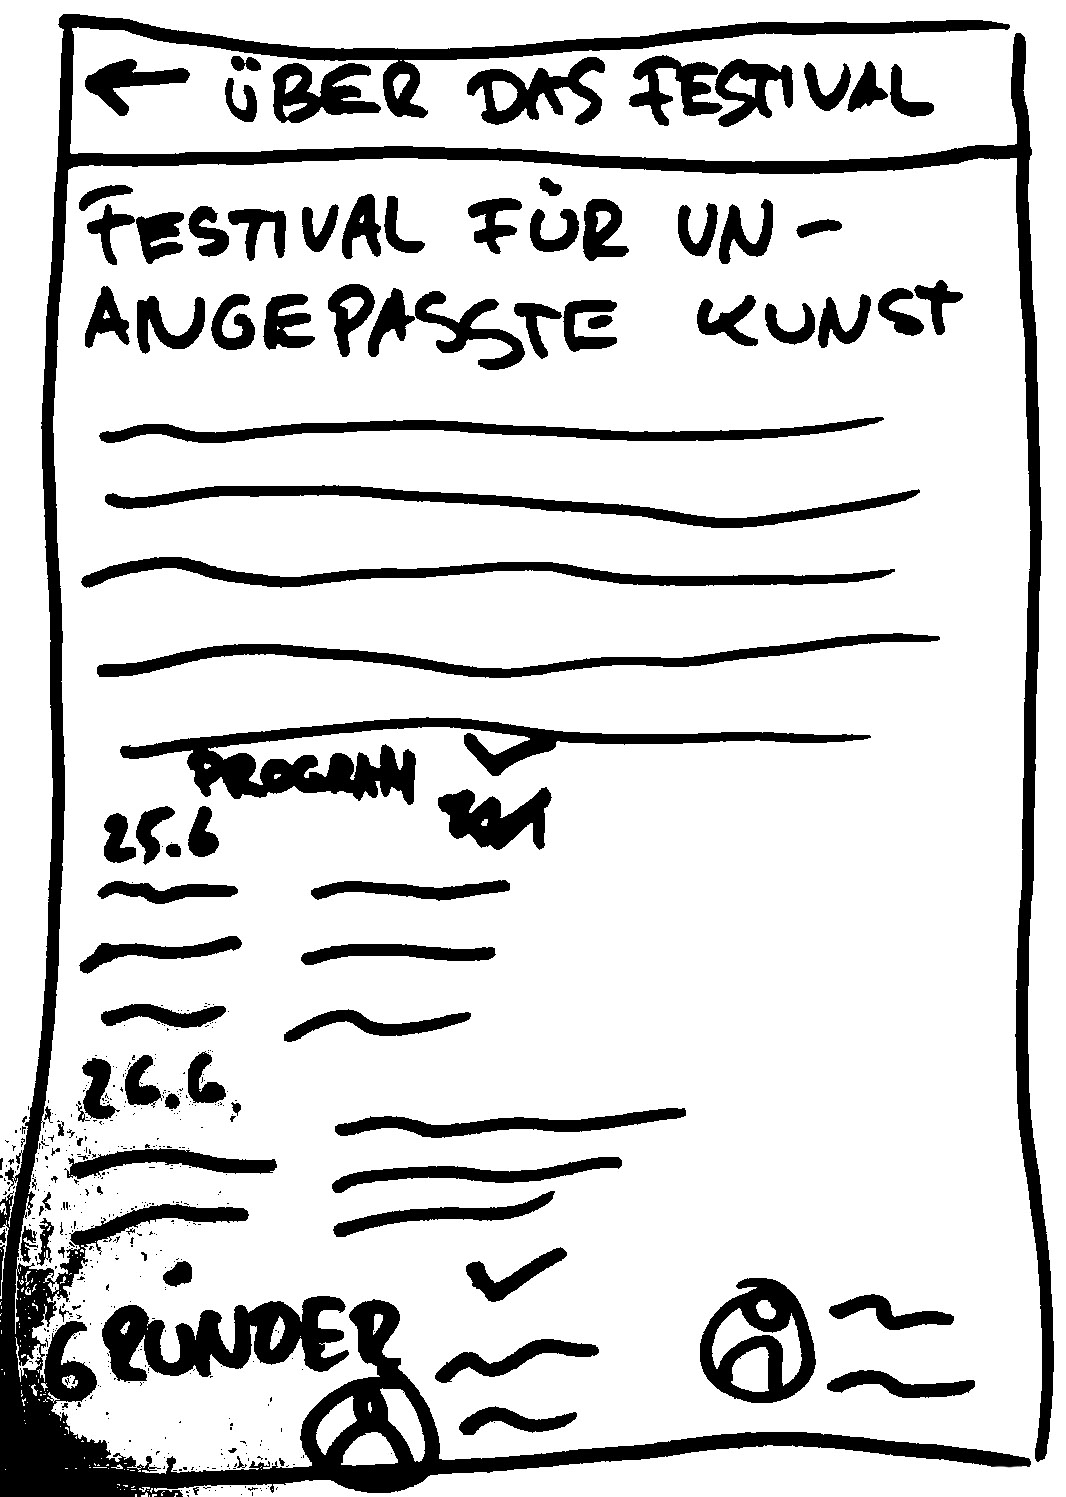
\includegraphics[width=\textwidth]{figures/festival-infos.jpg}
        \caption{Festival Informationen}
        \label{fig:gull}
    \end{subfigure}
    \begin{subfigure}[b]{0.22\textwidth}
        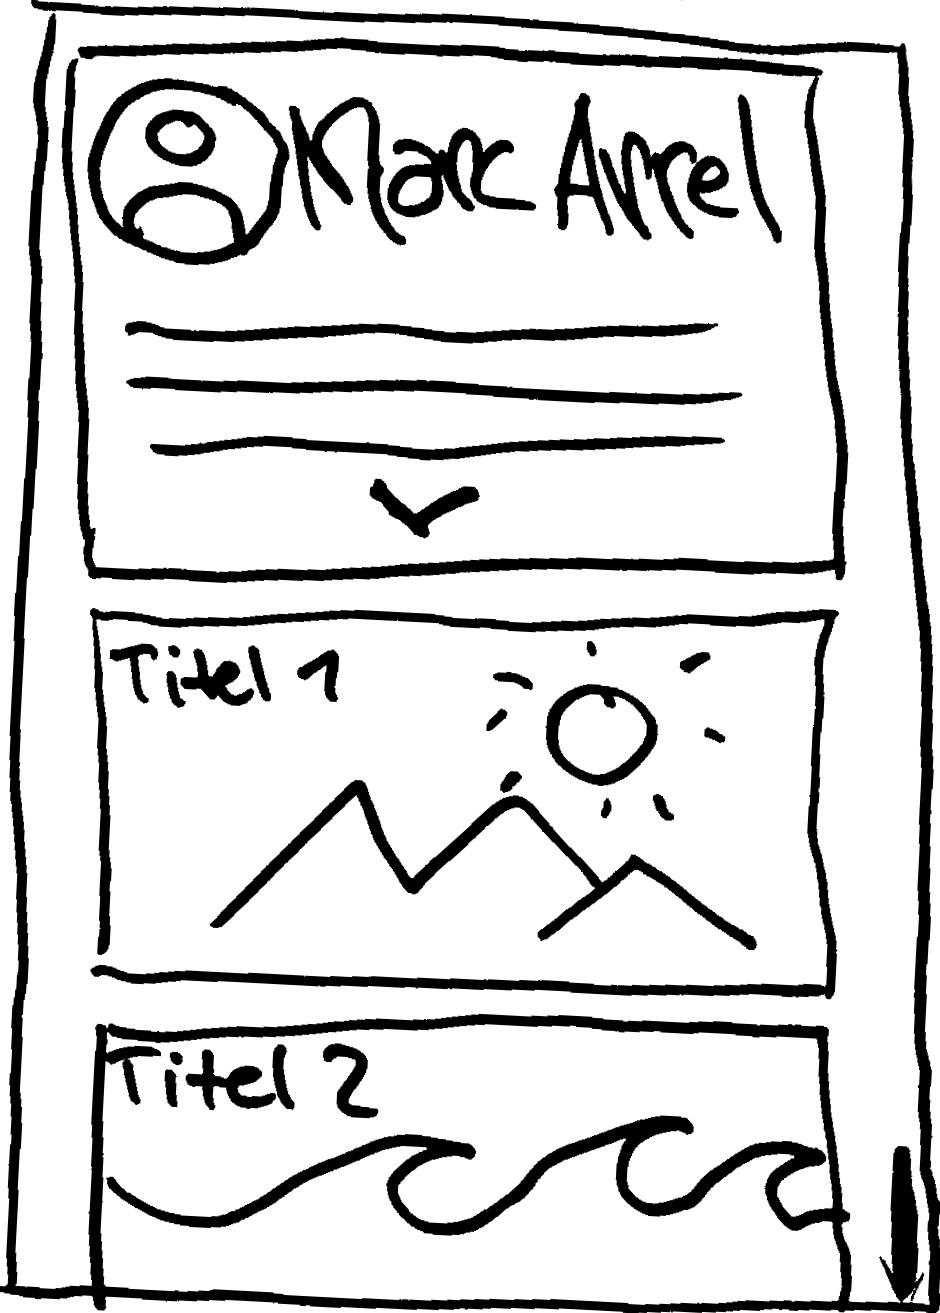
\includegraphics[width=\textwidth]{figures/kuenstler.jpg}
        \caption{Künstler Ansicht}
        \label{fig:tiger}
    \end{subfigure}
    \caption{Zwei unserer Skizzen}
    \label{fig:skizzen}
\end{figure}
\subsection{Klick-Prototyp}
Mit den Einsichten aus den Skizzen und dem Paper Prototype haben wir einen \textit{high-fidelity} Klick-Prototyp erstellt. Dazu wurden Wireframes von allen Ansichten in Adobe Photoshop oder Adobe Illustrator erstellt. Diese wurden dann in Invision\footnote{\url{https://www.invisionapp.com/}} hochgeladen. Hier können die einzelnen Ansichten verknüpft und animiert werden. So entsteht ein Prototyp, der der finalen  App sehr ähnlich ist und der über einen Link von allen Teammitglieder aufgerufen, getestet und kommentiert werden kann. Dadurch konnten wir weitere Schwächen und Unzulänglichkeiten der Gestaltung erkennen und ausbessern.
\subsection{Entwicklung}
Zuletzt haben wir die Anwendung in Android implementiert. Als Entwicklungsumgebung wurde Android Studio verwendet, die Versionskontrolle erfolgte in Git. Natürlicherweise haben wir auch noch während der Entwicklung sowohl konzeptionelle als auch technische Probleme im Design gefunden, die ausgebessert werden mussten.
\section{Visuelle Gestaltung}

\section{Ansichten und Funktionen}

\section{Technische Details}

\section{Zusammenfassung}


\balance{} 

% \bibliographystyle{ACM-Reference-Format-Journals}
\bibliographystyle{SIGCHI-Reference-Format}
% \bibliographystyle{acm}
\bibliography{sample}

\end{document}

%%% Local Variables:
%%% mode: latex
%%% TeX-master: t
%%% End:
